\subsection{Plane strain confined compression}
\label{subsec:Me1}

\subsubsection{Definition}
\label{subsubsec:Me1_def}

This example deals with numerical analyses of a part of the whole rock mass based on special conditions concerning symmetry, structure of the rock mass and material behavior. In order to simulate an initial state of stress in different depths, a pressure at least at one boundary has to be applied which represents the load of the overburden. In addition to this the stresses decrease with depth because of the gravity and the density of the rock mass (Fig. \ref{Me_fme:cfound}).
\begin{figure}[!htb]
  \begin{center}
    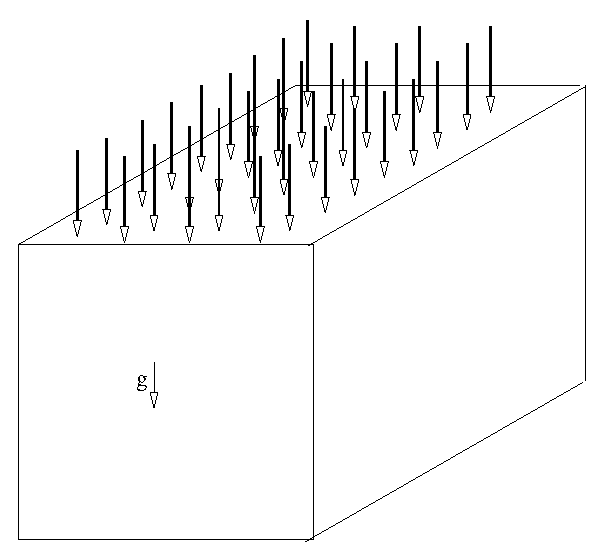
\includegraphics[scale=0.45]{PART_II/M/ex_plate_model.eps}
  \end{center}
  \caption{Conceptual model of elastic foundation}
  \label{Me_fme:cfound}
\end{figure}

\vspace*{-2.5ex}
\subsubsection{Solution}
\label{subsubsec:Me1_sol}

The calculation area has the size of $50\,\mbox{m}\times 50\,\mbox{m}$ (length and height), and the problem is simplified under plane strain conditions. The quadrilateral mesh is illustrated in Fig.~\ref{Me_fme:block}, which is refined in one corner in order to be used directly to conduct subsequently an elastic excavation simulation.

Regarding boundary conditions, a uniformly distributed pressure of $23.75\,\mbox{MPa}$ is prescribed for the top boundary. Such kind of boundary conditions are so called tractions in the context of mechanics, and they are treated as Neumann type boundary conditions. Boundary conditions are illustrated in more detail in Fig.~\ref{Me_fme:e1bc}.

Homogeneous material properties are assumed within the whole domain. Table \ref{Me_tme:el2d} represents the corresponding material parameters.

\clearpage

\begin{figure}[!htb]
  \centering
   \subfigure[FE mesh]{
   \includegraphics[width=0.46\textwidth]{PART_II/M/e1_mesh.eps}
   \label{Me_fme:block}}                
   \subfigure[Boundary conditions]{
   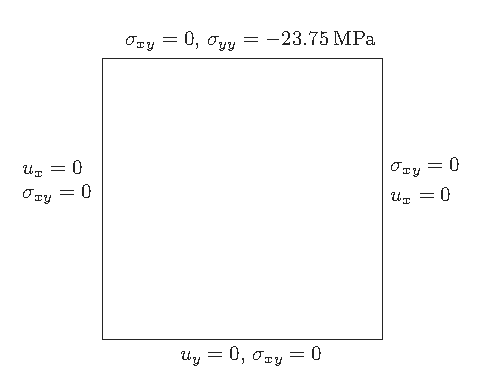
\includegraphics[width=0.46\textwidth]{PART_II/M/e1_bc.eps}
   \label{Me_fme:e1bc}}
  \caption{Finite element model. Left: Spatial discretization (1150 quadrilateral elements, 1101 nodes); Right: Boundary conditions}
  \label{Me_fme:meshbc}
\end{figure}

\begin{table}[!htb]
\centering
\caption{Material parameters}
\label{Me_tme:el2d}
\begin{tabular}{llll}
\toprule
Symbol & Parameter & Value & Unit \\
\midrule
$E$    & Young's modulus & $25$   & GPa \\
$\nu$  & Poisson's ratio & $0.3$  & -- \\
$\rho$ & Density         & $2500$ & kg$\cdot$m$^{-3}$ \\
\bottomrule
\end{tabular}
\end{table}

For this simple elastic problem, the following analytical solution exists:
\begin{equation}
 \stress_{yy} = -23.75-\dens h
  \label{Me_eq:ex1_ana}
\end{equation}
where $\dens$ is the solid density and $h$ is the height from top to bottom boundary.

\subsubsection{Results}
\label{subsubsec:Me1_res}

Fig.~\mbox{\ref{Me_fme:e1_syy} (left)} shows the distribution of vertical stress in the domain, which implies that the discretization error is very small. Fig.~\mbox{\ref{Me_fme:e1_syy} (right)} shows a linear variation of stress $\stress_{yy}$ along with height.
\begin{figure}[!thb]
  \begin{center}
  \epsfig{figure=PART_II/M/e1_uy.eps,width=6cm, height=6cm}
  \epsfig{figure=PART_II/M/ex1_plate_profile.eps,width=6cm, height=6cm}
  \end{center}
  \caption{Result of vertical stress, $\stress_{yy}$ (MPa). Left: domain distribution. Right: Vertical profile}
  \label{Me_fme:e1_syy}
\end{figure}

The numerical result of $\stress_{yy}$ at the bottom boundary is $-24.97\,\mbox{MPa}$, which is very close to the analytic solution, $\stress_{yy}=-25.0\,\mbox{MPa}$.
